\begin{frame}{Spannbäume – Beispiel Jarník-Prim}
	\centering
	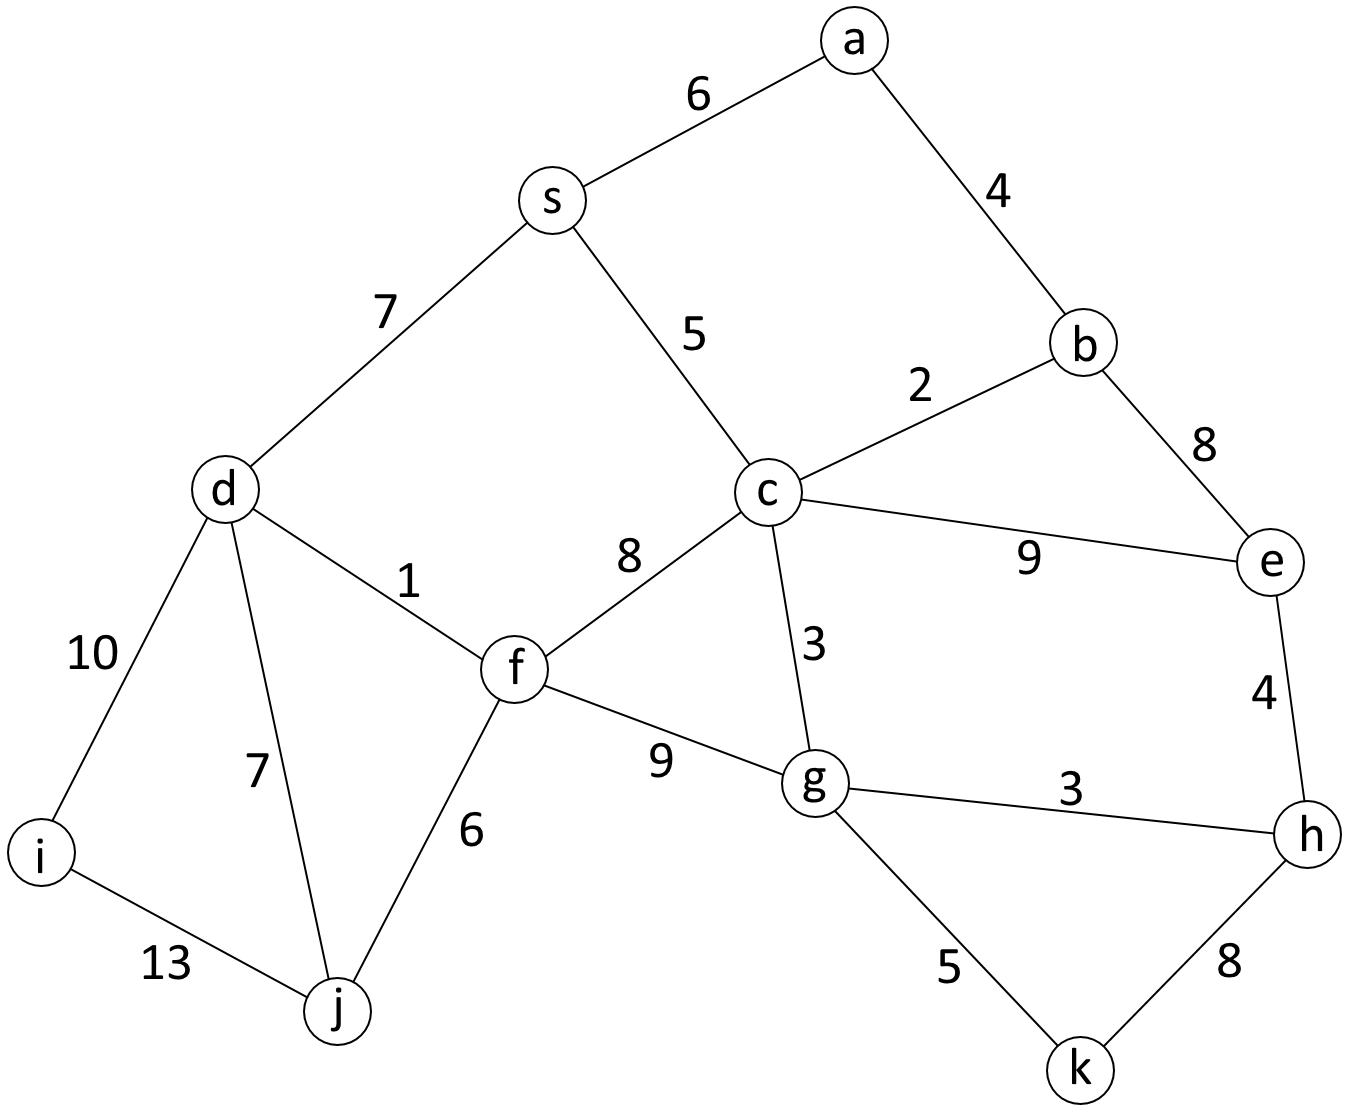
\includegraphics[width=.75\textwidth]{beispielgraph} \\
	\vspace{-.3\baselineskip}\hyperlink{label:afterEx1}{Hier klicken, um das Beispiel zu überspringen.}
\end{frame}

\begin{frame}{Spannbäume – Beispiel Jarník-Prim}
	
		\centering
		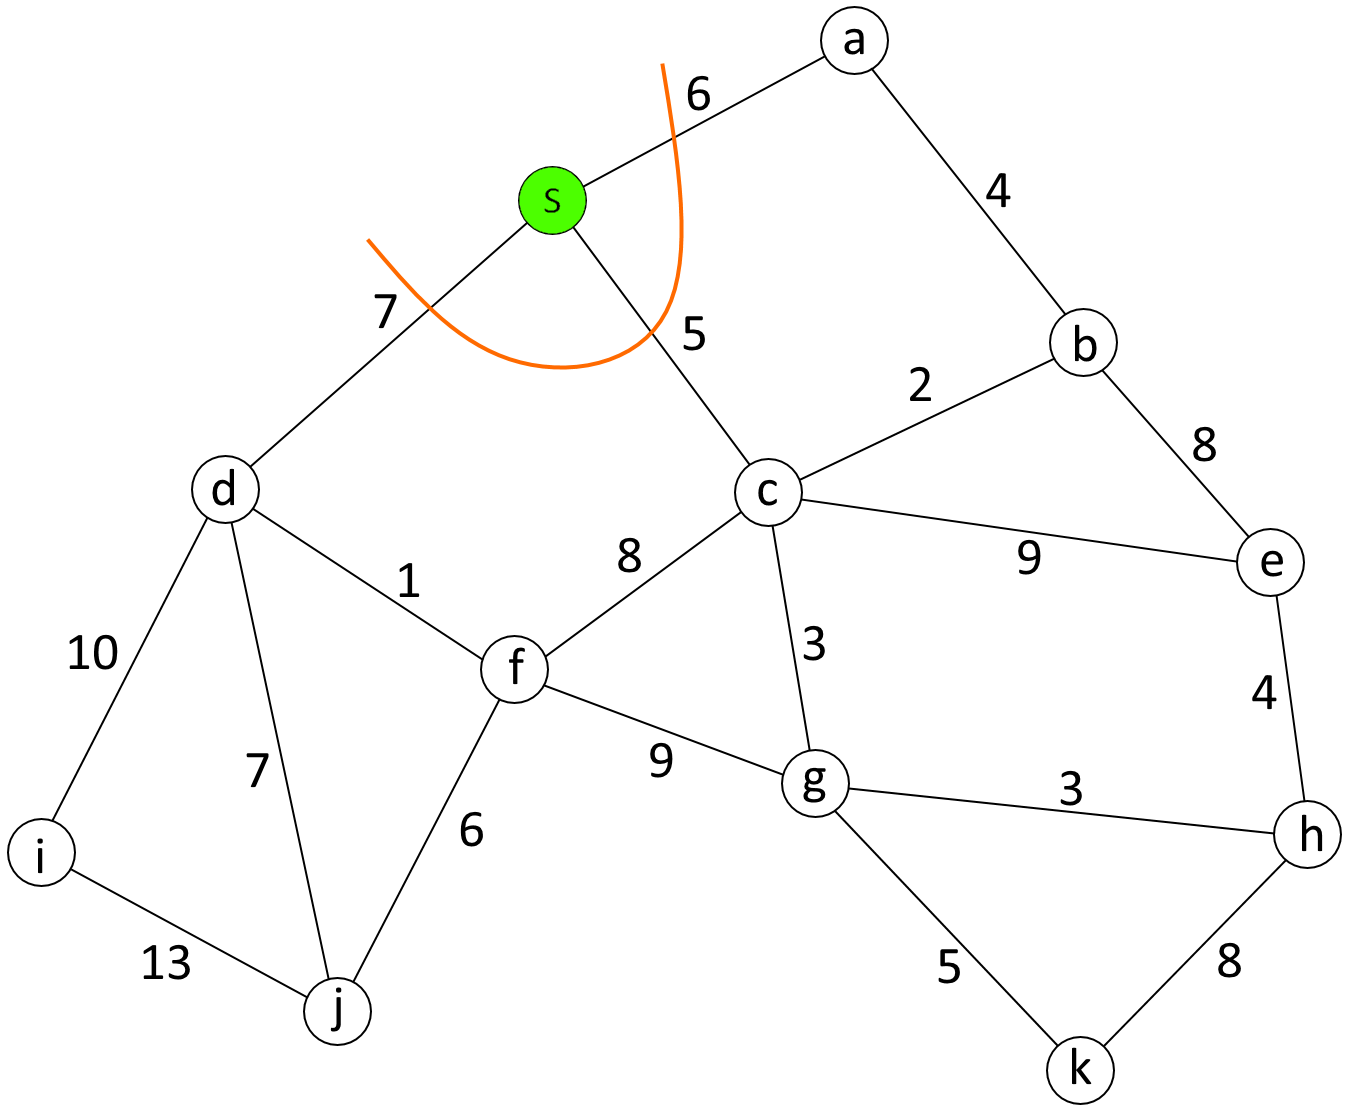
\includegraphics[width=.75\textwidth]{jp1}
	
\end{frame}

\begin{frame}{Spannbäume – Beispiel Jarník-Prim}
	
		\centering
		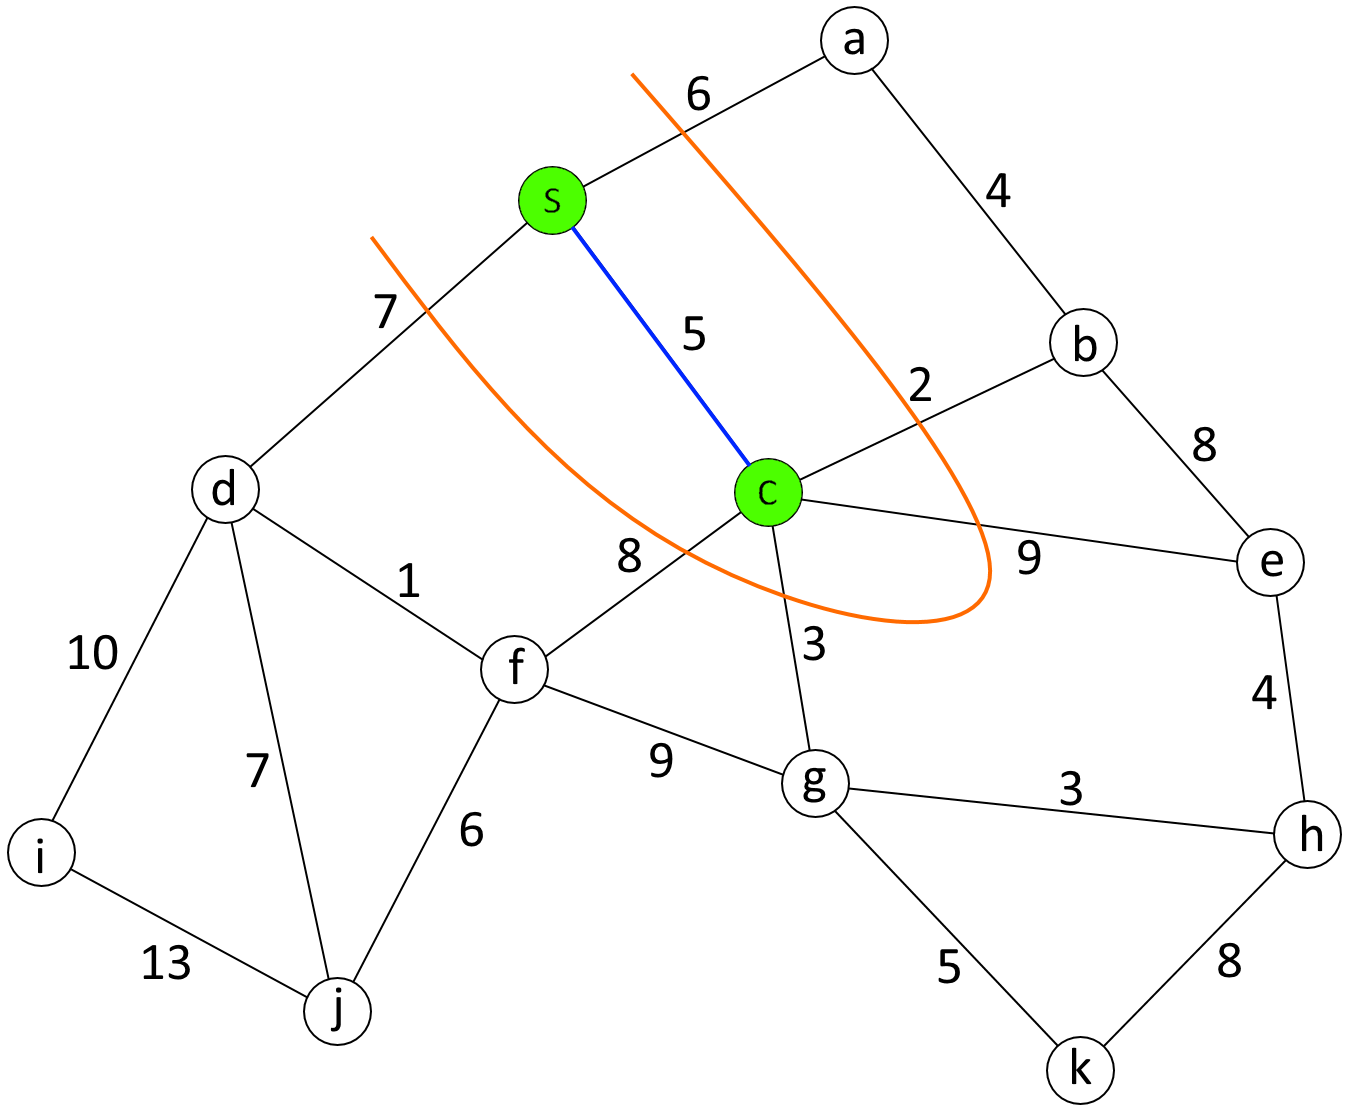
\includegraphics[width=.75\textwidth]{jp2}
	
\end{frame}

\begin{frame}{Spannbäume – Beispiel Jarník-Prim}
	
		\centering
		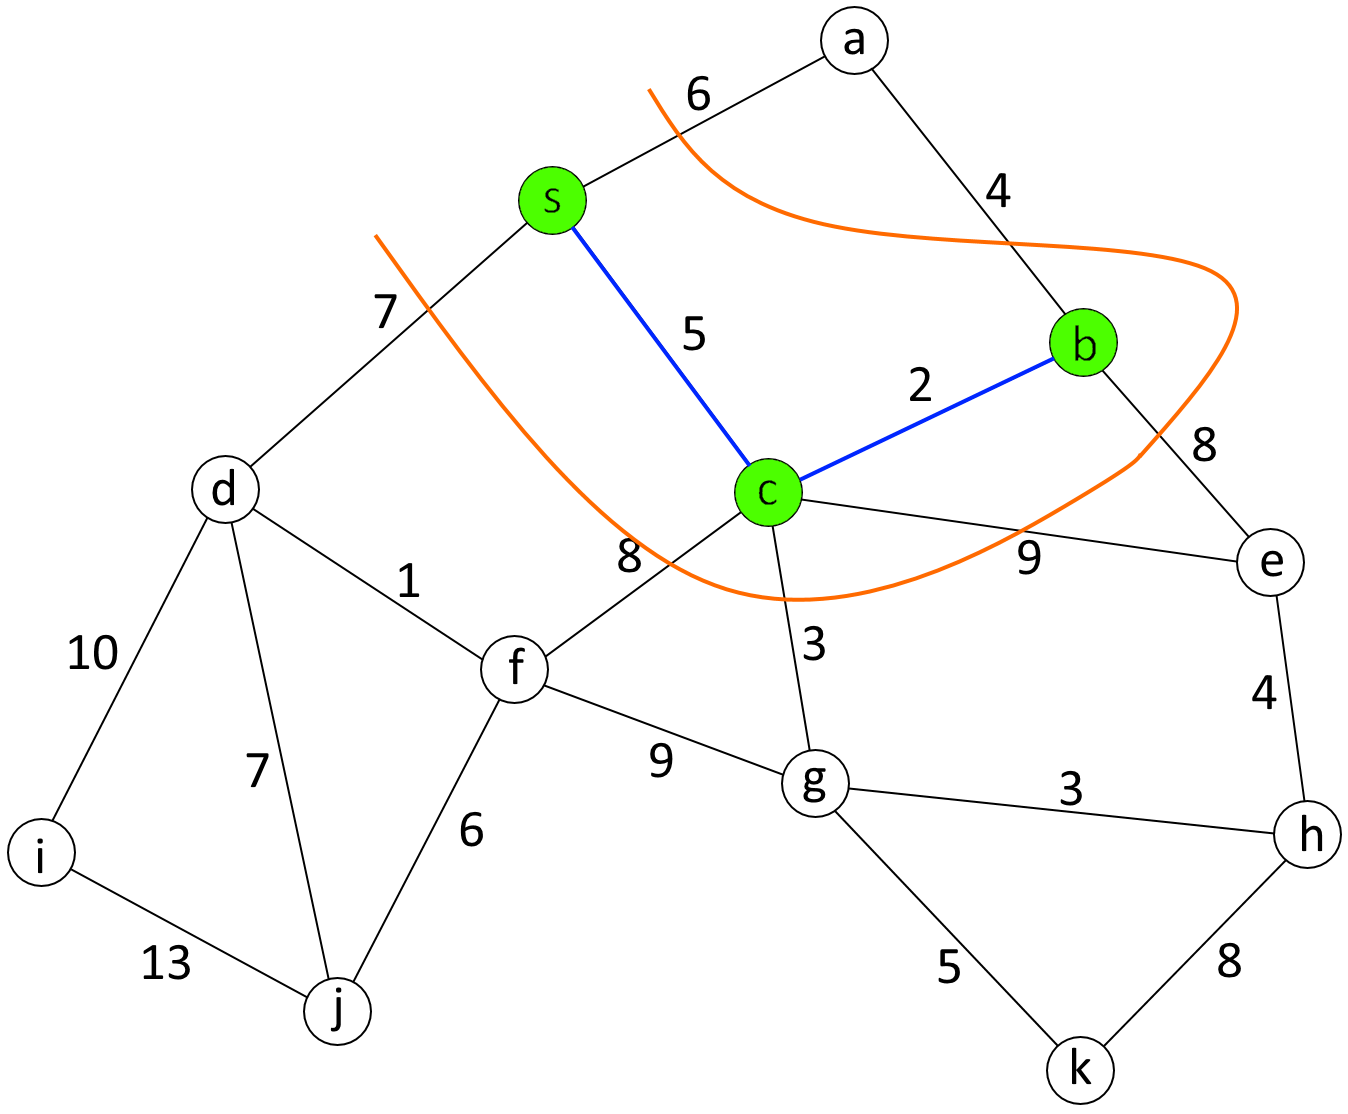
\includegraphics[width=.75\textwidth]{jp3}
	
\end{frame}

\begin{frame}{Spannbäume – Beispiel Jarník-Prim}
	
		\centering
		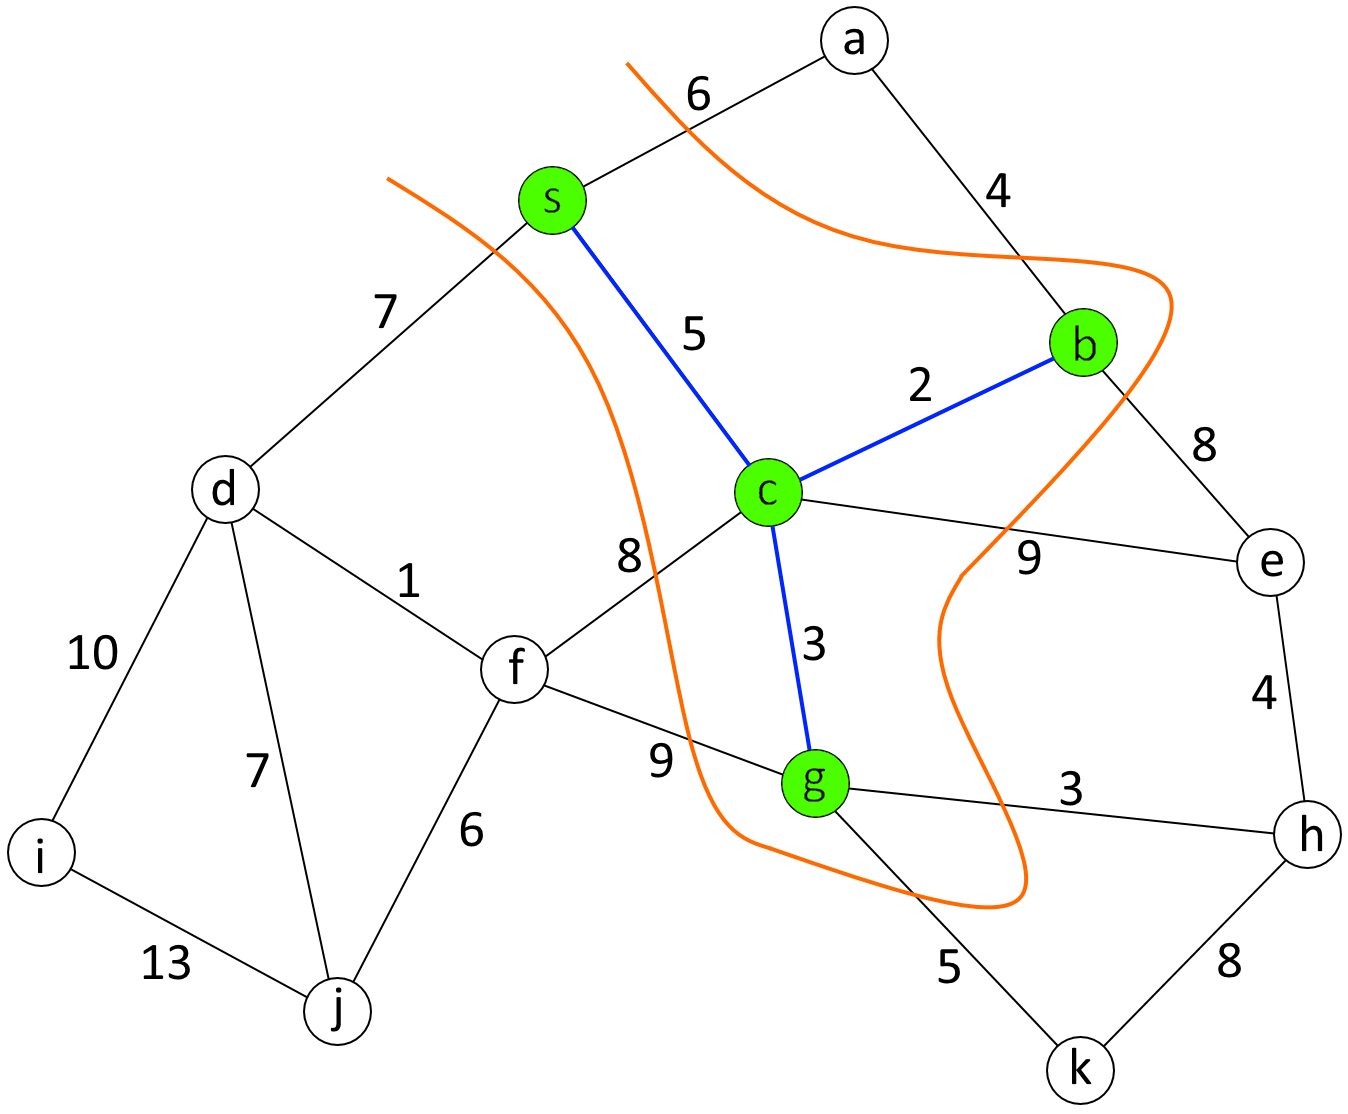
\includegraphics[width=.75\textwidth]{jp4}
	
\end{frame}

\begin{frame}{Spannbäume – Beispiel Jarník-Prim}
	
		\centering
		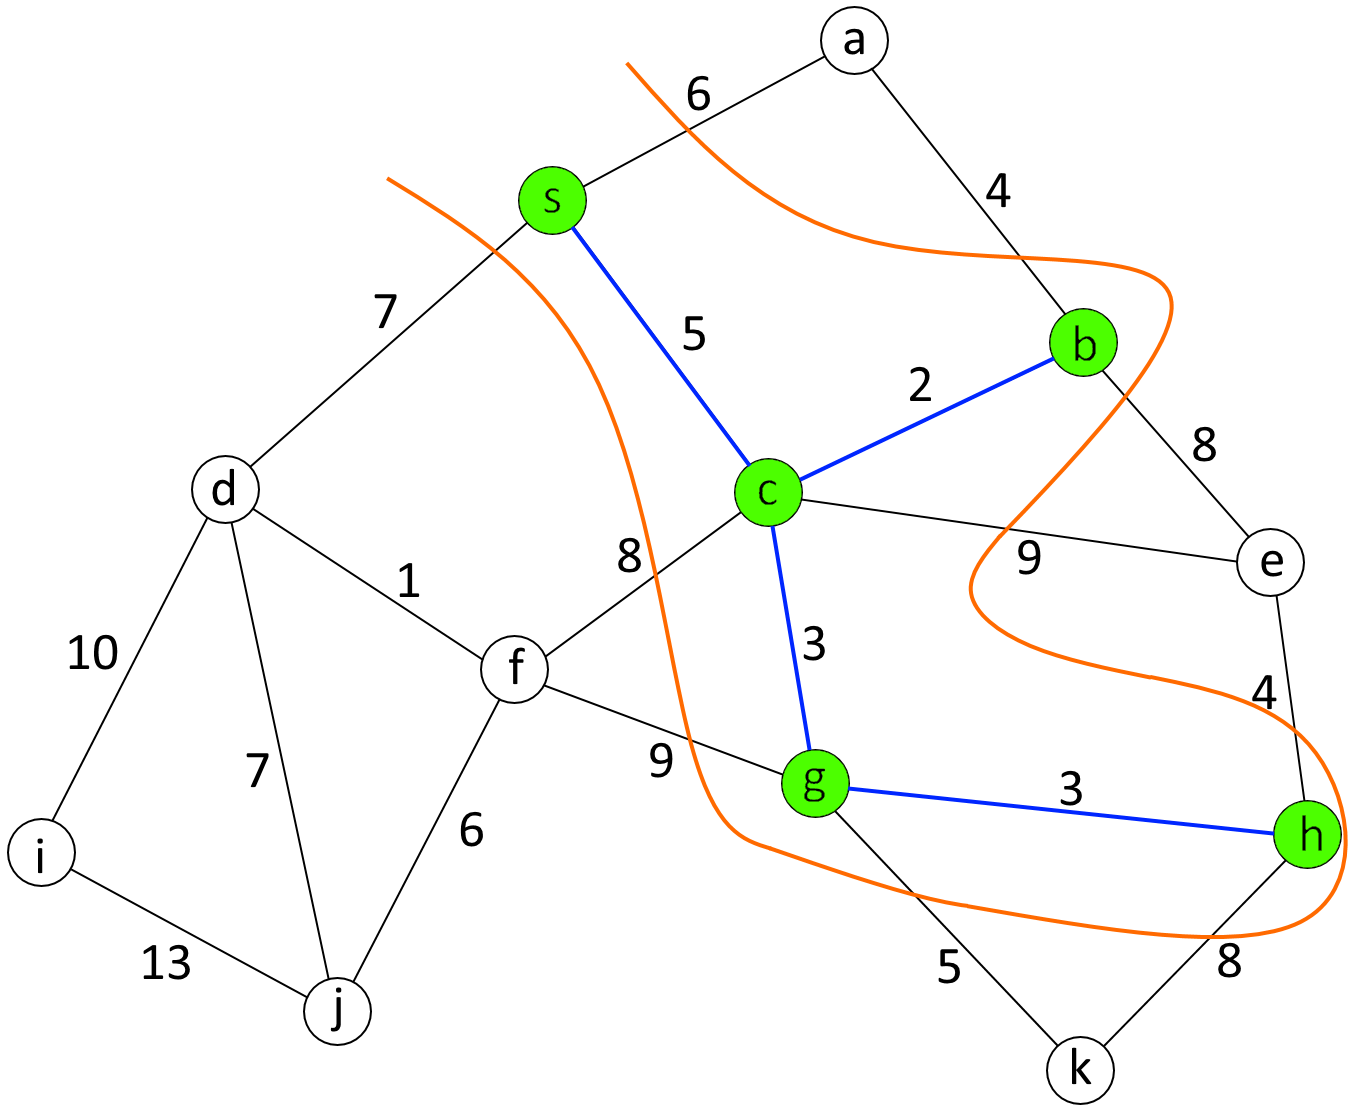
\includegraphics[width=.75\textwidth]{jp5}
	
\end{frame}

\begin{frame}{Spannbäume – Beispiel Jarník-Prim}
	
		\centering
		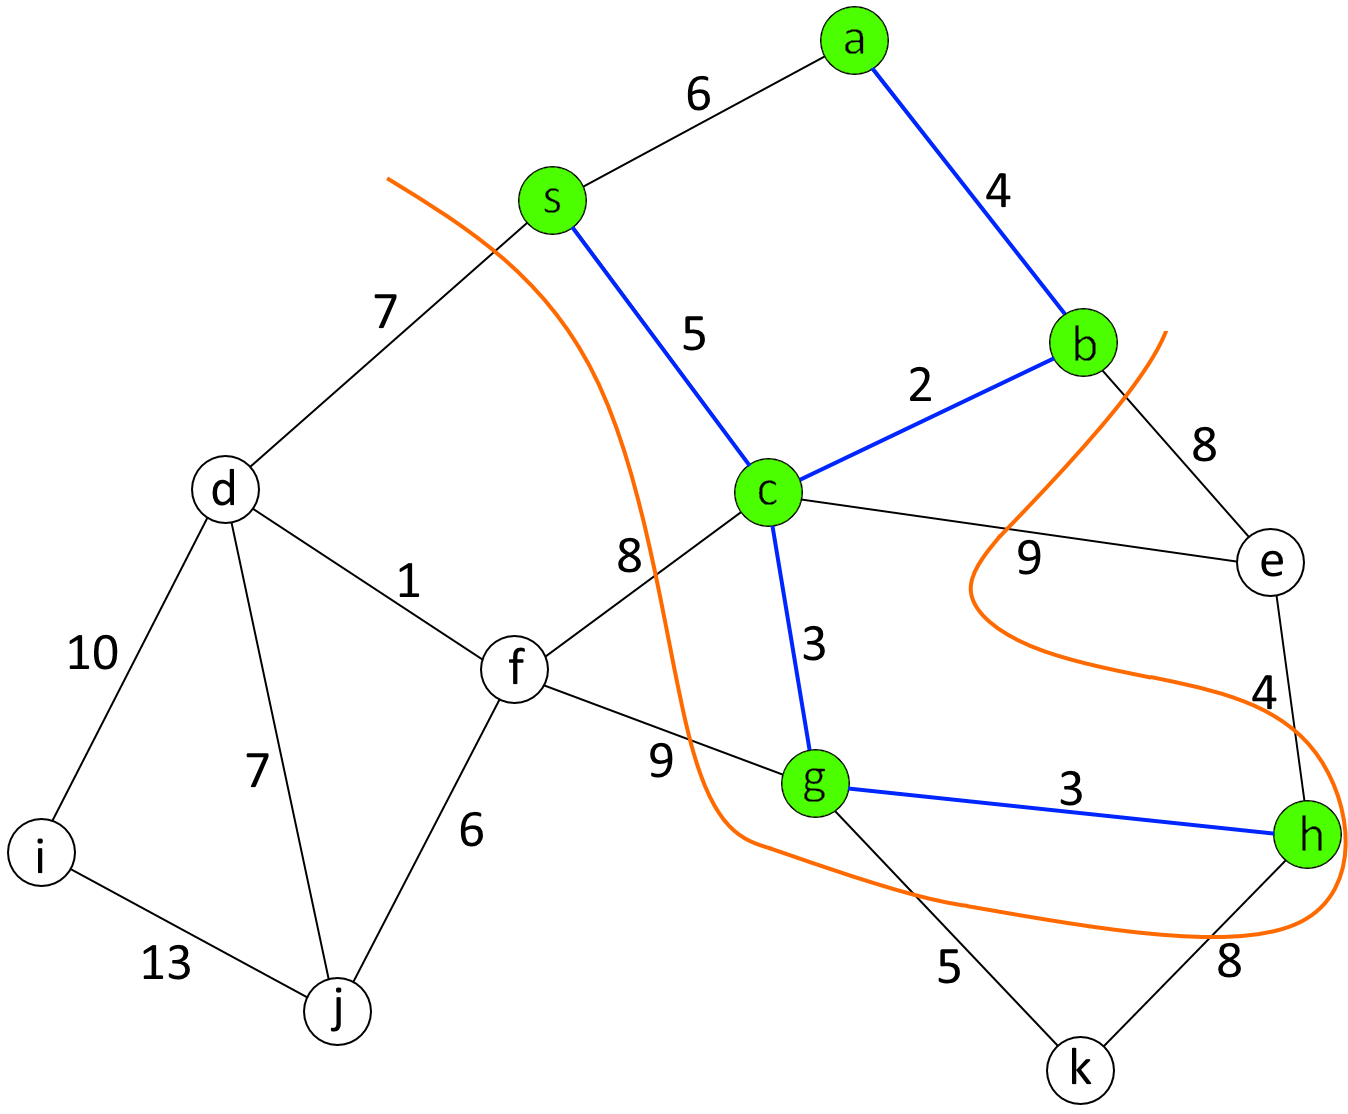
\includegraphics[width=.75\textwidth]{jp6}
	
\end{frame}

\begin{frame}{Spannbäume – Beispiel Jarník-Prim}
	
		\centering
		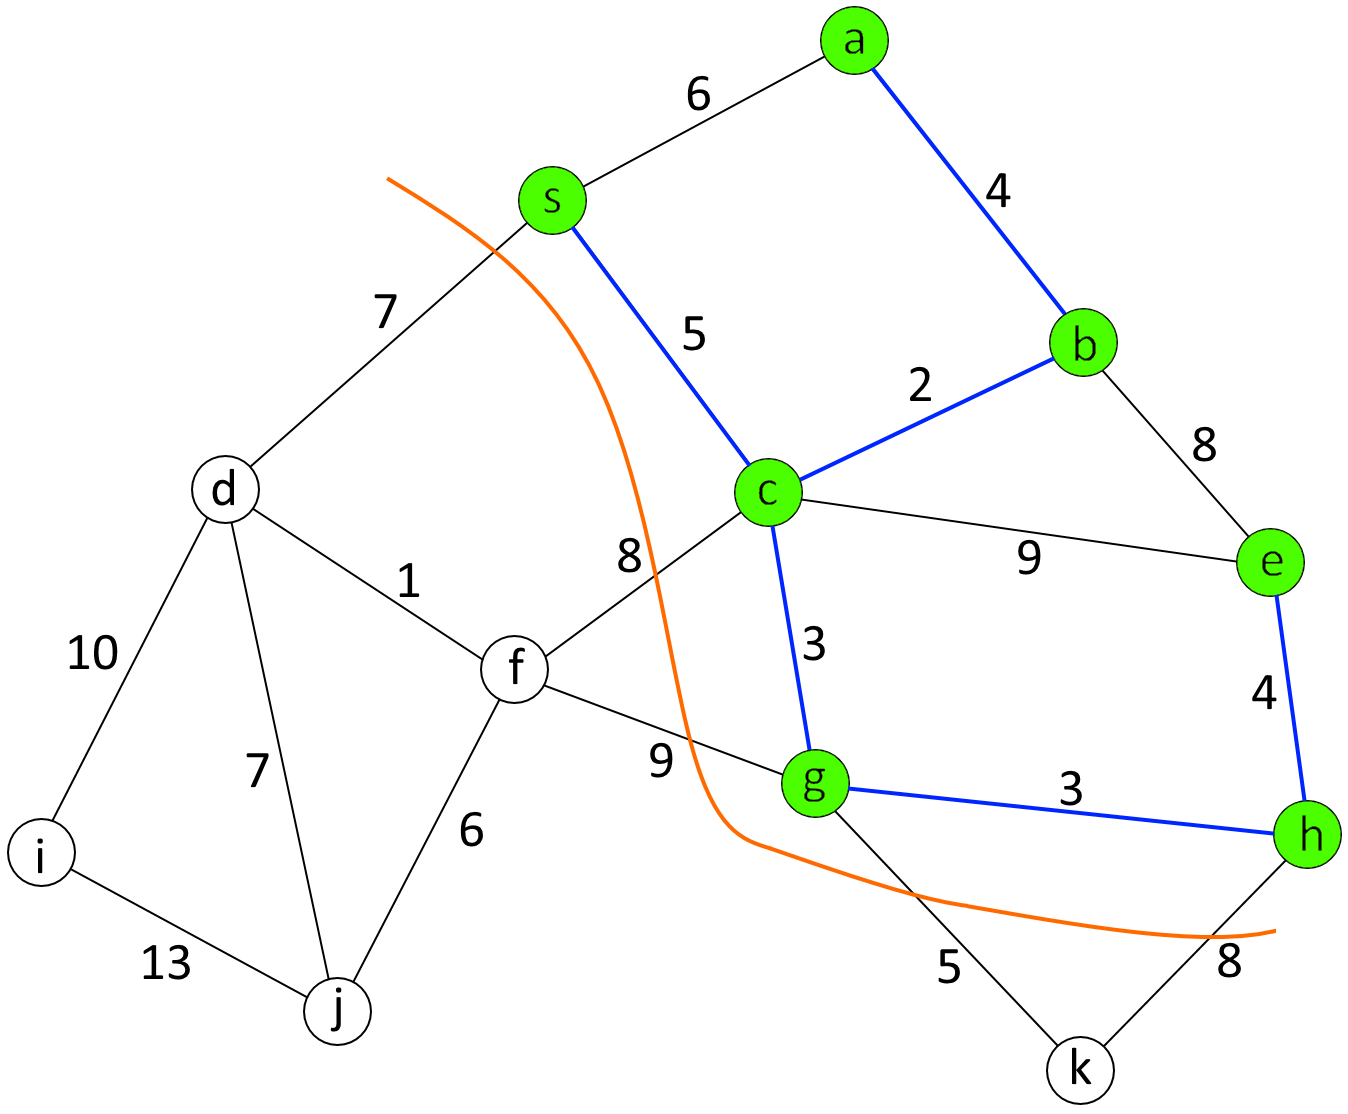
\includegraphics[width=.75\textwidth]{jp7}
	
\end{frame}

\begin{frame}{Spannbäume – Beispiel Jarník-Prim}
	
		\centering
		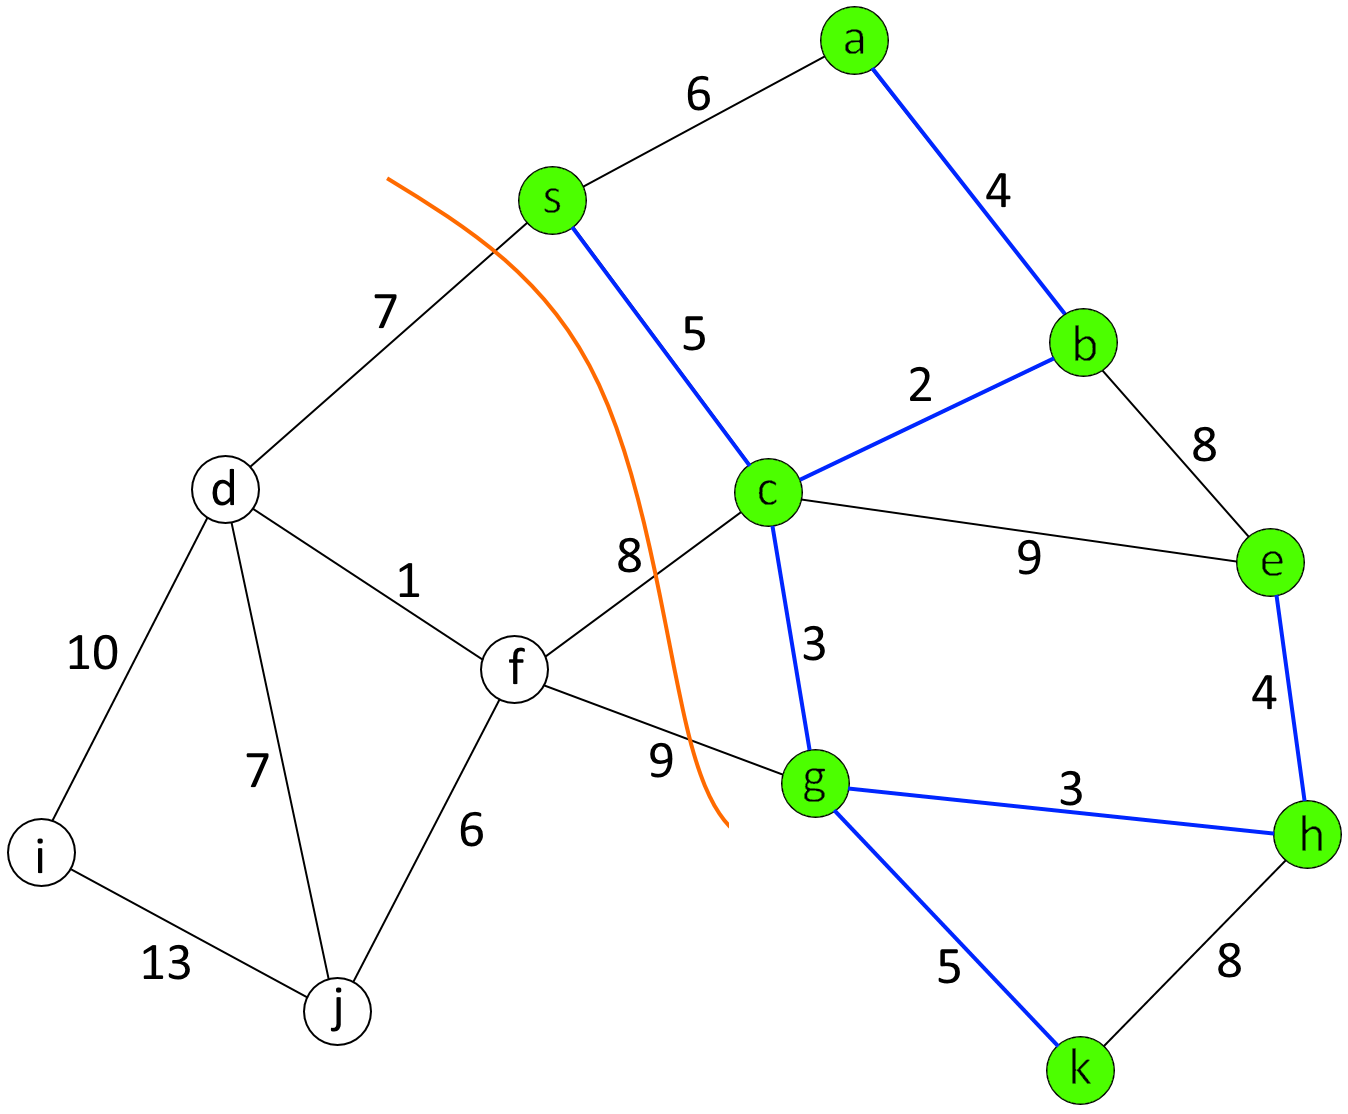
\includegraphics[width=.75\textwidth]{jp8}
	
\end{frame}

\begin{frame}{Spannbäume – Beispiel Jarník-Prim}
	
		\centering
		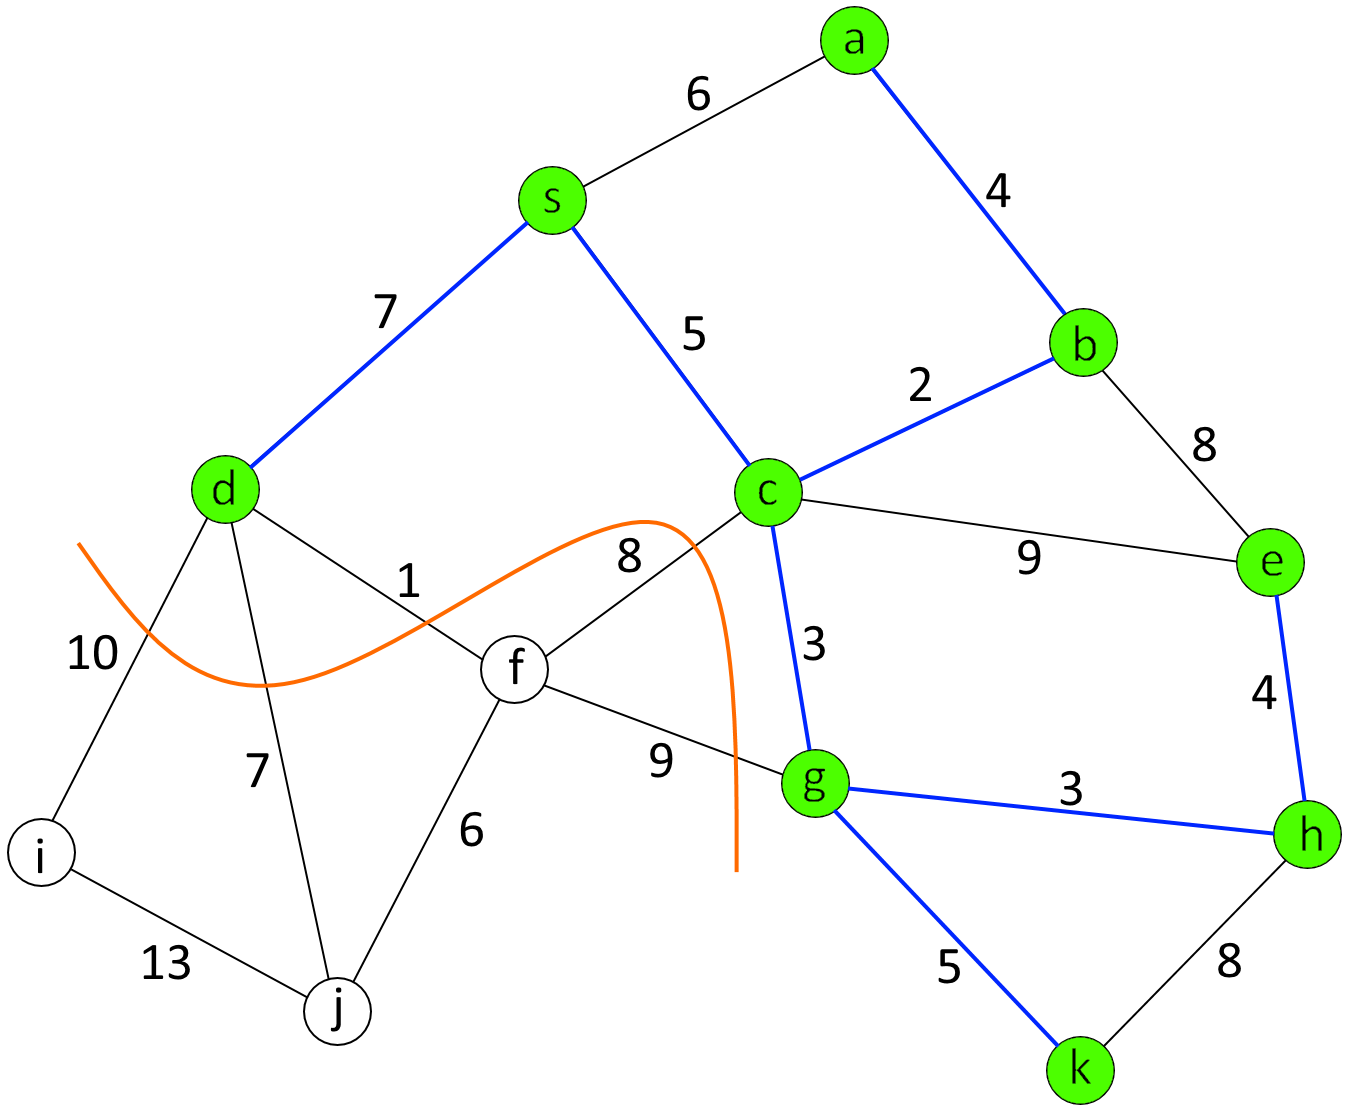
\includegraphics[width=.75\textwidth]{jp9}
	
\end{frame}

\begin{frame}{Spannbäume – Beispiel Jarník-Prim}
	
		\centering
		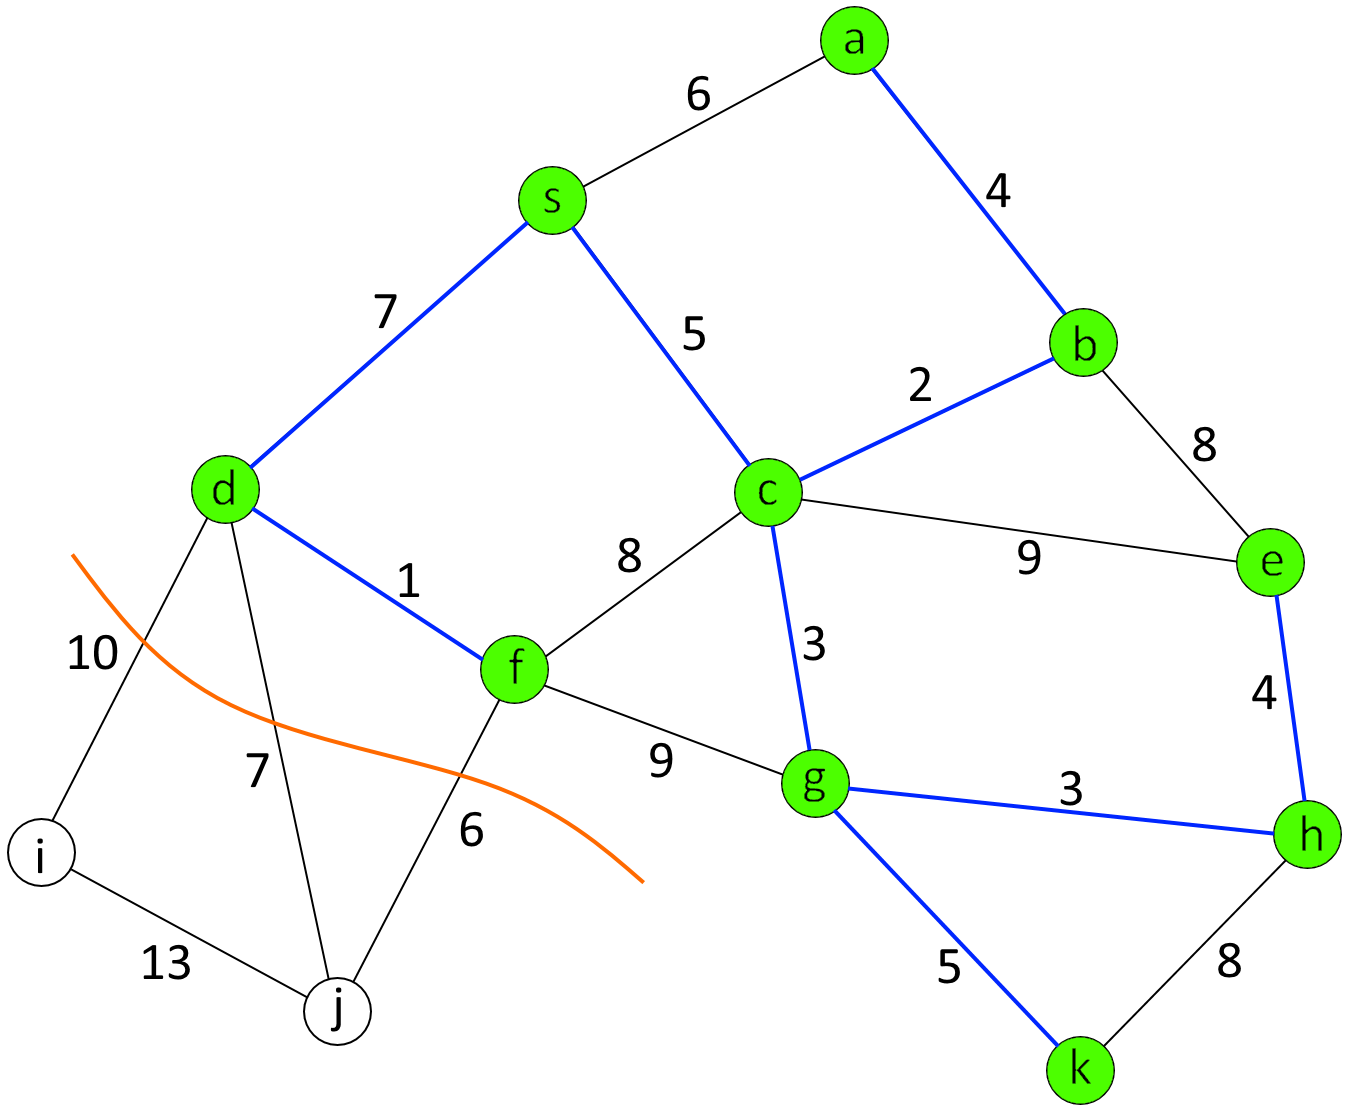
\includegraphics[width=.75\textwidth]{jp10}
	
\end{frame}

\begin{frame}{Spannbäume – Beispiel Jarník-Prim}
	
		\centering
		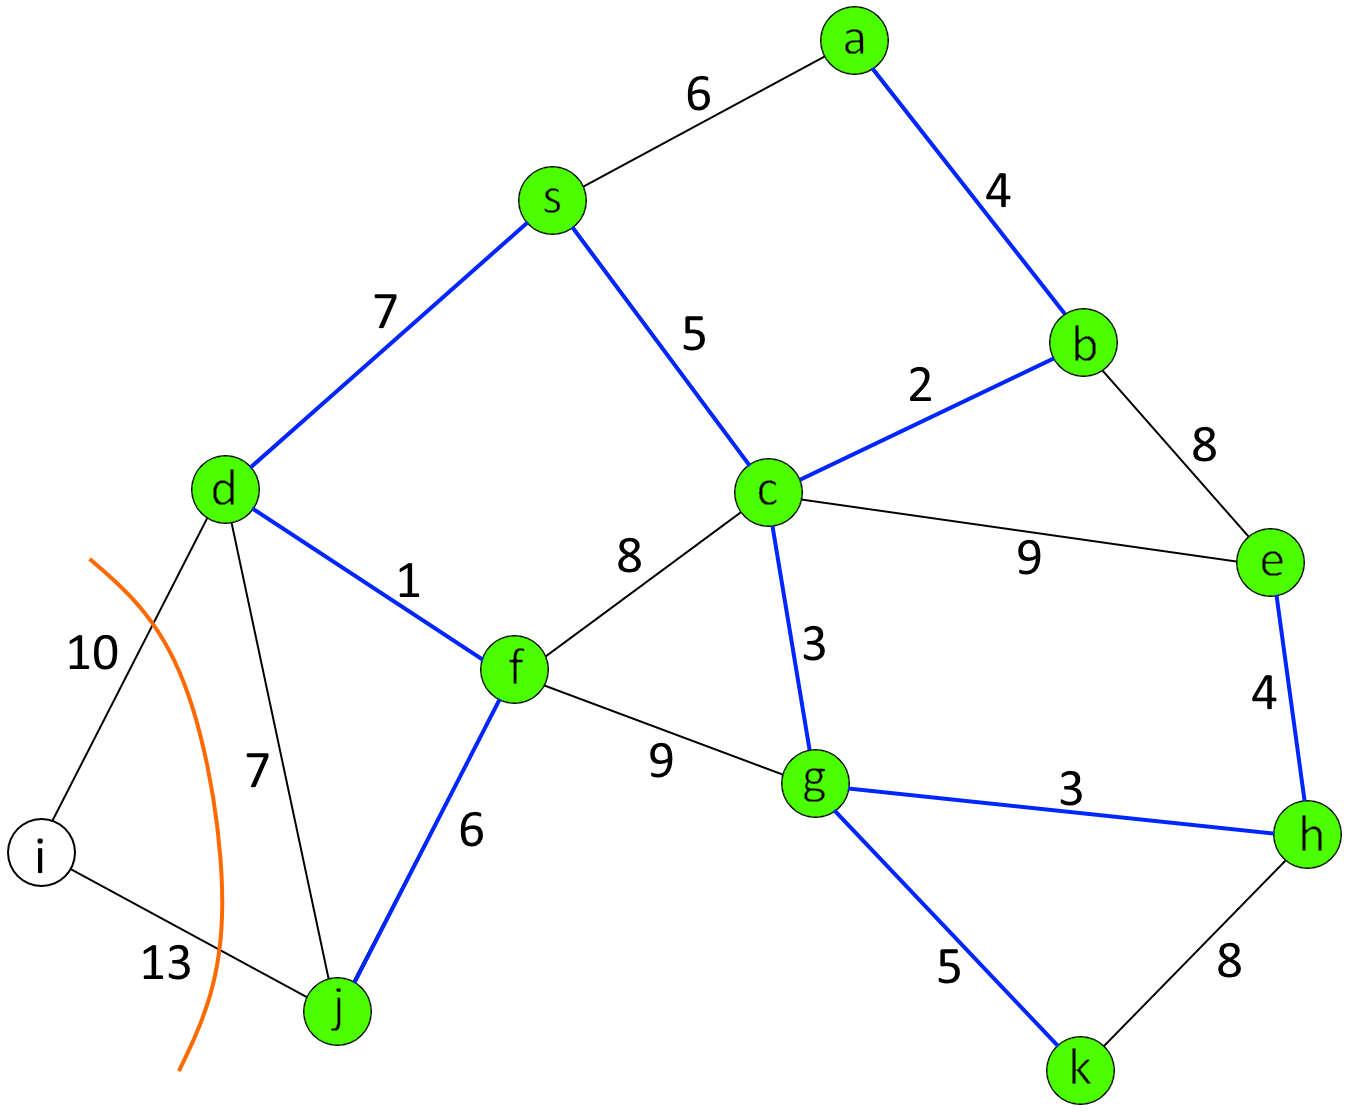
\includegraphics[width=.75\textwidth]{jp11}
	
\end{frame}

\begin{frame}{{\hypertarget{label:afterEx1}{}Spannbäume – Beispiel Jarník-Prim}}
		\centering
		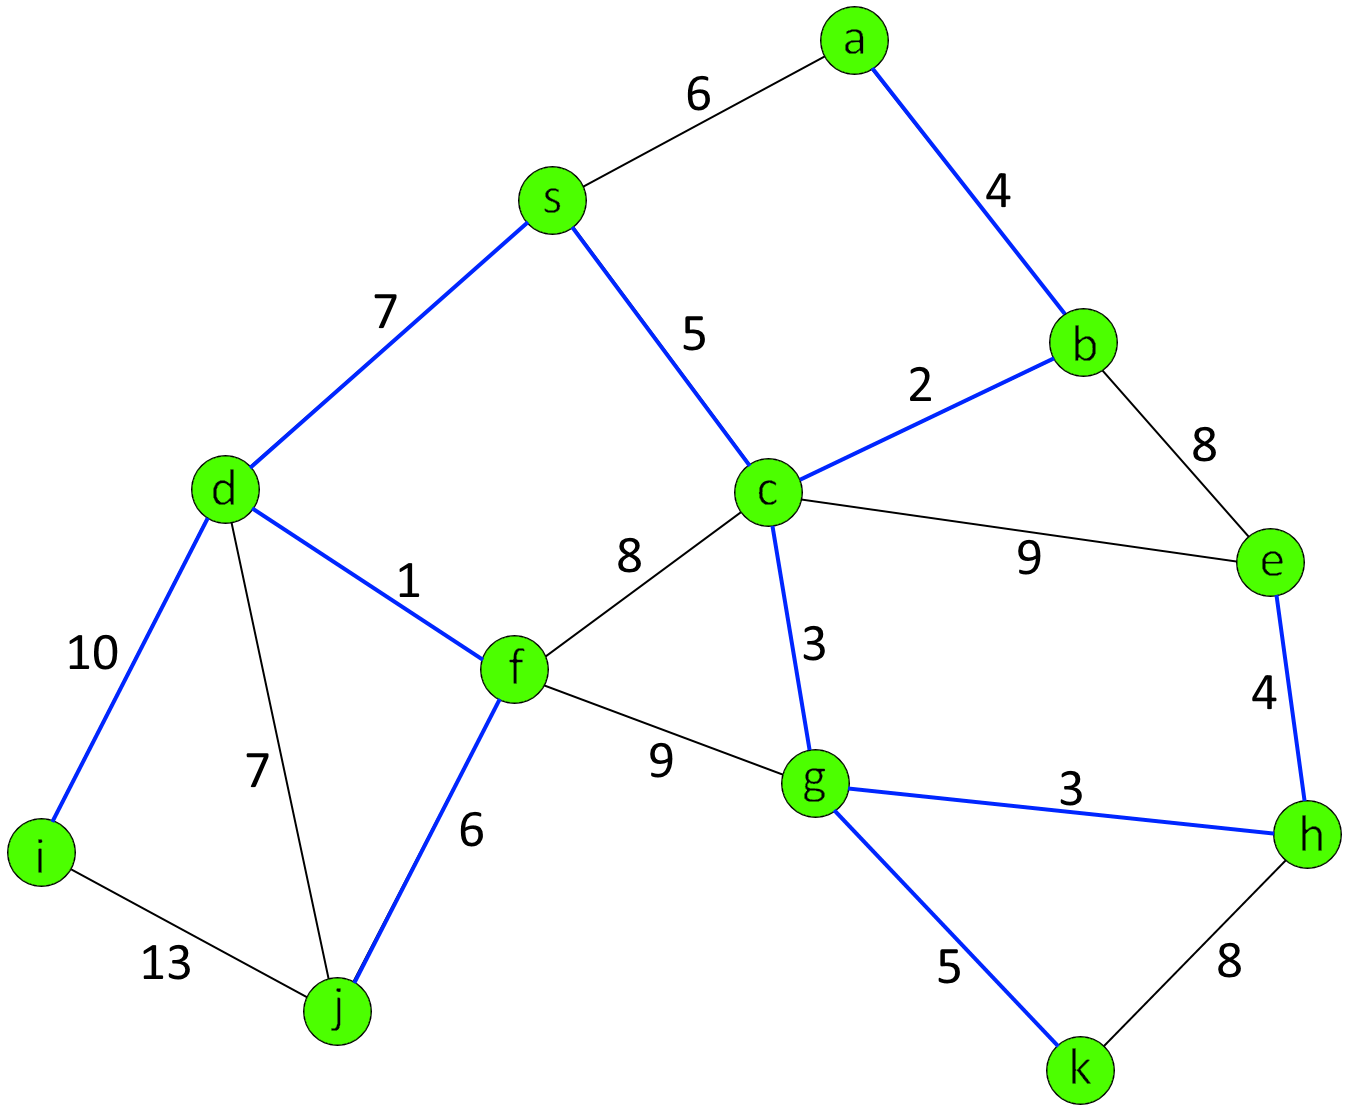
\includegraphics[width=.75\textwidth]{jp12}
\end{frame}